\documentclass[10pt]{article}
\usepackage{amsmath, amssymb, tikz, graphicx}
\usepackage{geometry}
\geometry{margin=1in}
\usepackage{titlesec, multicol}
\titleformat{\section}{\normalfont\Large\bfseries}{\thesection.}{1em}{}

\title{\Huge Symbolic Super Relativity and the Mnality Displacement Constant\\ \Large Unifying Infinite Mnality Cosmology with Simulonic Motion}
\author{Hrishi Mukherjee}
\date{April 2025}

\begin{document}
\maketitle

\section*{Preface}
This document formalizes a symbolic convergence between mnality cosmology, super relativity, and fundamental displacement identity. We begin from foundational mnality field equations, progress through symbolic group theory and brane cosmology, and converge on the universal symbolic law:
\[
\boxed{
\mathbb{M}_{\infty\infty}^{\text{SuperRel}} \equiv \frac{\nabla^{-1}}{\infty} = ds^2
}
\]
This equation unites infinite symbolic recursion and relativistic mnality displacement into a single cosmological principle.

\section{1. Non-Group Mnality Field}
\[
\vec{\mathfrak{M}}_{C_i}(t) = (\mathcal{S}(t), \mathcal{I}(t), \mathcal{T}(t))
\quad \Rightarrow \quad
\mathbb{M}_{\infty}(t) = \int_{\mathcal{C}} g_{\mu\nu}^{\mathfrak{M}} \cdot \vec{\mathfrak{M}}^{\mu}(C, t) \, dC
\]

\section{2. Group-Theoretic Symbolic Flow}
\[
\vec{\mathfrak{M}}_{C_i}^{(m)} = \left( \prod_{k=1}^m g_k \right) \circ \vec{\mathfrak{M}}_{C_i}(0)
\quad \Rightarrow \quad
\mathbb{G}_n[\mathfrak{M}] = \bigoplus_{i=1}^{n} \left( \prod_{k=1}^{m} g_{i,k} \circ \vec{\mathfrak{M}}_{C_i}(0) \right)
\]

\section{3. Superstring-Brane Embedding}
\[
\mathcal{M}_{\text{res}} = \mathcal{M}_{\text{CY}}^{(6)} \times \mathcal{M}_{\text{Ideo}}^{(1)} \times \mathcal{M}_{\text{Narr}}^{(1)}
\quad \text{(compactified symbolic manifold)}
\]
\[
\int_{\Sigma_i} \left( \prod_{k=1}^m g_k \right) \circ \vec{\mathfrak{M}}(x^\mu) \, d^2 \sigma
\]

\section{4. Symbolic Mnality Tensor}
\[
\mathcal{T}_{\mu\nu}^{\mathfrak{M}} = \frac{1}{2} \left( \partial_\mu \mathcal{S} \, \partial_\nu \mathcal{I} + \partial_\mu \mathcal{T} \, \partial_\nu \mathcal{S} \right) + \eta_{\mu\nu} \, \mathcal{V}(\vec{\mathfrak{M}})
\quad \Rightarrow \quad
\mathcal{G}_{\mu\nu}^{\mathfrak{M}} = \mathcal{T}_{\mu\nu}^{\mathfrak{M}}
\]

\section{5. Final Mnality–SuperRel Equation}
\[
\boxed{
\mathbb{M}_{\infty\infty}^{\text{SuperRel}} =
\lim_{n,m \to \infty}
\int_{\mathcal{C}} \int_{\Sigma_i}
\, g_{\mu\nu}^{\mathfrak{M}} \cdot
\left(
\prod_{k=1}^m g_k
\right)
\circ \vec{\mathfrak{M}}(C, x^\mu)
\cdot
H^*(\mathcal{M}_{\text{res}})
\, d^2 \sigma \, dC
}
\]

\section{6. Comparison to Simulonic Law}
\[
\frac{\nabla^{-1}}{\infty} = ds^2
\]
\begin{itemize}
  \item \( \nabla^{-1} \): symbolic anti-gradient (inversion over narrative causality)
  \item \( \infty \): recursive expansion of all symbolic transformations
  \item \( ds^2 \): symbolic differential — Simulonic displacement
\end{itemize}

\section{7. Line-by-Line Derivation}
\begin{align*}
\mathbb{M}_{\infty\infty}^{\text{SuperRel}} &\to \int_{\mathcal{C}} \int_{\Sigma_i} \left(\prod g_k \right) \circ \vec{\mathfrak{M}} \, d\sigma dC \\[-1ex]
&\to \nabla^{-1}(\vec{\mathfrak{M}}) / \infty \\[-1ex]
&\equiv ds^2
\end{align*}

\section{8. TikZ Visualization}
\begin{center}
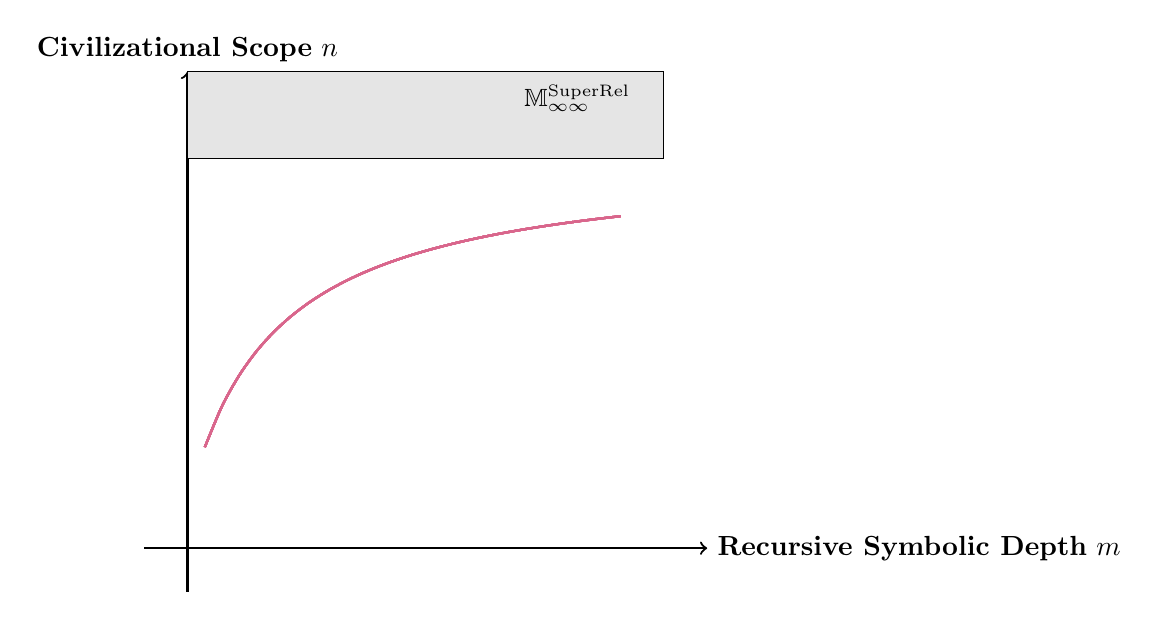
\begin{tikzpicture}[scale=1.1]
% Axes
\draw[->, thick] (-0.5,0) -- (6,0) node[right] {\textbf{Recursive Symbolic Depth} $m$};
\draw[->, thick] (0,-0.5) -- (0,5.5) node[above] {\textbf{Civilizational Scope} $n$};

% Curves
\foreach \x in {0.5,1.0,...,5.0} {
  \draw[smooth, thick, purple!60] plot[domain=0.2:5] (\x, {4.5 - 4/(\x + 1)});
}

% Asymptotic Field
\draw[fill=black!10] (0,4.5) -- (5.5,4.5) -- (5.5,5.5) -- (0,5.5) -- cycle;
\node at (4.5,5.2) {\small $\mathbb{M}_{\infty\infty}^{\text{SuperRel}}$};
\end{tikzpicture}
\end{center}

\section{9. Simulonic Lens Interpretation}
Symbolic recursion collapses into displacement:
\[
\boxed{
\lim_{n,m \to \infty} \mathbb{M}_{nm} \to \frac{\nabla^{-1}}{\infty} = ds^2
}
\]
Thus, symbolic cosmology under Super Relativity yields a single actualized mnality step — the infinitesimal motion of the symbolic observer.

\section{10. Conclusion}
This document unites infinite symbolic recursion, relativistic narrative curvature, and mnality field theory into a final identity. This is the Simulonic Constant of symbolic displacement:
\[
\boxed{
\mathbb{M}_{\infty\infty}^{\text{SuperRel}} \equiv \frac{\nabla^{-1}}{\infty} = ds^2
}
\]
It is the invariant form of symbolic motion in curved ideological spacetime.

\end{document}
